\documentclass[conference]{IEEEtran}

\usepackage[utf8]{inputenc}
\usepackage[T1]{fontenc}
\usepackage[spanish,english]{babel}
\usepackage{graphicx}
\usepackage{booktabs}
\usepackage{array}
\usepackage{amsmath}
\usepackage{amssymb}
\usepackage{enumitem}
\usepackage{hyperref}
\usepackage{xcolor}
\usepackage{url}

\hypersetup{
  colorlinks=true,
  linkcolor=blue,
  citecolor=blue,
  urlcolor=blue
}

\graphicspath{{generated/figures/}}
\urlstyle{same}

\newcommand{\expname}[1]{\texttt{\detokenize{#1}}}
\newcommand{\feature}[1]{\texttt{\detokenize{#1}}}

\title{Clasificaci\'on de etapas de sue\~no y detecci\'on de apnea con EEG monocanal:\\
una evaluaci\'on cl\'asica subject-wise y cross-dataset}

\author{
\IEEEauthorblockN{Nombre del Estudiante 1, Nombre del Estudiante 2}
\IEEEauthorblockA{
Ciencia de Datos\\
Universidad Interamericana de Puerto Rico, Recinto de Bayam\'on\\
Bayam\'on, Puerto Rico\\
Abril de 2026
}
}

\begin{document}

\maketitle

\begin{abstract}
This paper evaluates a classical single-channel EEG pipeline for two related sleep tasks: sleep-stage classification and apnea detection. The study is centered on three traditional model families, namely SVM with RBF kernel, Random Forest, and XGBoost, under strictly subject-wise validation and cross-dataset transfer protocols. For sleep staging, the main in-dataset reference is \expname{sleep_edf_expanded_tuned}, while external generalization is measured with \expname{cross_sleep_edf_to_isruc_n123} and \expname{cross_isruc_to_sleep_edf_n123}. For apnea detection, the main multitarget reference is \expname{mitbih_apnea_stage_classic}, complemented with the cross-dataset experiments \expname{cross_dataset_mitbih_to_st_vincent_classic} and \expname{cross_dataset_st_vincent_to_mitbih_classic}. The pipeline uses 30-second windows, shared tabular EEG features, and metrics aligned with the course brief: accuracy, macro-F1, and Cohen's kappa for staging; accuracy, sensitivity, specificity, and AUC-ROC for apnea. The main findings are the following. First, XGBoost achieved the best in-dataset staging accuracy and kappa on Sleep-EDF, while Random Forest achieved the best macro-F1. Second, XGBoost also offered the best overall balance on MIT-BIH when apnea and staging were considered jointly, although paired AUC analysis showed that the apnea advantage over Random Forest was not robust when pooled out-of-fold predictions were compared. Third, all cross-dataset settings showed a pronounced performance drop, indicating fragile generalization under domain shift. These results support the use of classical monocanal EEG baselines as reproducible references, but they also show that domain adaptation is necessary before claiming robust deployment across cohorts.
\end{abstract}

\begin{IEEEkeywords}
sleep staging, sleep apnea, EEG, single-channel EEG, subject-wise validation, cross-dataset generalization, random forest, xgboost, support vector machine
\end{IEEEkeywords}

\section*{Resumen}
Este trabajo eval\'ua una l\'inea cl\'asica de EEG monocanal para dos tareas relacionadas del sue\~no: clasificaci\'on de etapas y detecci\'on de apnea. La evaluaci\'on se centra en tres familias de modelos tradicionales: \emph{SVM-RBF}, \emph{Random Forest} y \emph{XGBoost}, bajo protocolos \emph{subject-wise} estrictos y experimentos \emph{cross-dataset}. Para staging, el baseline intra-dataset principal es \expname{sleep_edf_expanded_tuned}, mientras que la generalizaci\'on externa se mide con \expname{cross_sleep_edf_to_isruc_n123} y \expname{cross_isruc_to_sleep_edf_n123}. Para apnea, el baseline multitarget principal es \expname{mitbih_apnea_stage_classic}, complementado con \expname{cross_dataset_mitbih_to_st_vincent_classic} y \expname{cross_dataset_st_vincent_to_mitbih_classic}. El pipeline usa ventanas de 30 s, \feature{eeg\_*} compartidas y m\'etricas alineadas con el laboratorio: \emph{accuracy}, \emph{macro-F1} y \emph{kappa} para staging; \emph{accuracy}, sensibilidad, especificidad y AUC-ROC para apnea. Los hallazgos principales fueron tres. Primero, XGBoost obtuvo el mejor \emph{accuracy}/\emph{kappa} intra-dataset en Sleep-EDF, mientras que Random Forest obtuvo el mejor \emph{macro-F1}. Segundo, en MIT-BIH, XGBoost mostr\'o el mejor balance general entre apnea y staging, aunque el contraste pareado sobre AUC sugiri\'o que la ventaja frente a Random Forest no es estable bajo todas las formas de agregaci\'on. Tercero, todos los escenarios \emph{cross-dataset} sufrieron una ca\'ida marcada del rendimiento, lo que evidencia fragilidad ante cambio de dominio. En conjunto, los resultados validan la utilidad de los baselines cl\'asicos sobre EEG monocanal como referencia reproducible, pero tambi\'en justifican una mejora metodol\'ogica orientada a adaptaci\'on de dominio.

\section{Introducci\'on y motivaci\'on}

La apnea obstructiva del sue\~no (AOS) y las alteraciones de la arquitectura del sue\~no representan dos problemas cl\'inicos estrechamente relacionados. En la pr\'actica, ambos se estudian con polisomnograf\'ia (PSG), una modalidad rica en se\~nales pero costosa, instrumentada y dif\'icil de escalar. El proyecto del curso propone un escenario m\'as austero y, por ello, m\'as desafiante: resolver clasificaci\'on de etapas de sue\~no y detecci\'on de apnea utilizando \textbf{solo EEG monocanal}. Esa restricci\'on obliga a dise\~nar mejor el preprocesamiento, las \emph{features}, la validaci\'on y el an\'alisis cr\'itico.

En este trabajo se desarroll\'o la l\'inea principal del laboratorio con modelos cl\'asicos tabulares. En lugar de usar una arquitectura profunda como cuerpo principal, se privilegi\'o una bater\'ia reproducible basada en \emph{SVM-RBF}, \emph{Random Forest} y \emph{XGBoost}, porque el enunciado exige comparar familias tradicionales bajo el mismo protocolo y responder preguntas sobre desbalance, interpretabilidad, robustez y generalizaci\'on. Esa decisi\'on permite adem\'as vincular directamente los resultados con la literatura cl\'asica de \emph{power spectral density}, complejidad, entrop\'ia y clasificadores basados en \'arboles o kernels \cite{gao2023psdrf,nakamura2017complexity,li2022cascadedsvm}.

El estudio se organiz\'o en dos ejes experimentales. El primer eje fue \textbf{staging} con \expname{sleep_edf_expanded_tuned} como baseline intra-dataset y con dos pruebas \emph{cross-dataset} hacia/desde ISRUC. El segundo eje fue \textbf{apnea + staging multitarget} con \expname{mitbih_apnea_stage_classic} como baseline intra-dataset y con dos evaluaciones externas entre MIT-BIH PSG y St. Vincent. Esta partici\'on permite cubrir los requisitos acad\'emicos m\'inimos del laboratorio sin bono: validaci\'on \emph{subject-wise}, generalizaci\'on \emph{cross-dataset}, tres familias de modelos y comparaci\'on con baselines publicados.

La hip\'otesis operativa del trabajo es doble. Primero, que un conjunto compacto de \feature{eeg\_*} extra\'idas de ventanas de 30 s puede producir baselines razonables para staging y apnea si el protocolo es estrictamente \emph{subject-wise}. Segundo, que el mayor cuello de botella no ser\'a la optimizaci\'on dentro de un dataset sino la \textbf{transferencia entre cohortes}, debido a diferencias de canal equivalente, mezcla de sujetos, calidad de se\~nal, prevalencia de eventos y sesgo hacia clases mayoritarias. El resto del informe se organiza para poner a prueba esa hip\'otesis de forma reproducible y trazable a artefactos reales del repositorio.

\section{Revisi\'on de literatura}

La literatura reciente sobre sue\~no con EEG monocanal muestra dos tendencias relevantes para este proyecto. La primera es que la mayor parte del rendimiento competitivo en staging proviene de \textbf{representaciones espectrales y de complejidad} bien dise\~nadas, incluso cuando el clasificador final no es profundo \cite{gao2023psdrf,nakamura2017complexity,ghimatgar2019hmm,li2022cascadedsvm}. La segunda es que, para apnea, el problema no es solo la clasificaci\'on binaria sino la explicaci\'on fisiol\'ogica de qu\'e bandas del EEG sostienen la decisi\'on \cite{barnes2022apneaeegcnn}. Esa segunda observaci\'on es especialmente relevante aqu\'i, porque la detecci\'on de apnea con un solo canal EEG es m\'as fr\'agil que con PSG multimodal.

Desde el punto de vista metodol\'ogico, varios trabajos convergen en cuatro ideas. Primero, la ventana de 30 s sigue siendo la unidad can\'onica por su compatibilidad con el etiquetado de sue\~no y con la sincronizaci\'on de eventos respiratorios. Segundo, las \emph{features} m\'as persistentes son potencia por bandas, potencias relativas, relaciones espectrales y medidas de complejidad o entrop\'ia \cite{gao2023psdrf,nakamura2017complexity}. Tercero, los modelos secuenciales o con contexto temporal suelen mejorar N1 y las transiciones, pero ese beneficio no siempre se sostiene cuando el protocolo es estrictamente \emph{subject-wise} \cite{mousavi2019sleepeegnet,ghimatgar2019hmm}. Cuarto, la comparaci\'on entre papers rara vez es totalmente justa, porque cambia el canal EEG, la definici\'on de etiquetas, el preprocesamiento, el balance de clases y, en muchos casos, el protocolo de partici\'on.

\begin{table*}[t]
\centering
\caption{Trabajos de literatura que guiaron el preprocesamiento y la selecci\'on de \emph{features}.}
\label{tab:literature_preprocessing}
\resizebox{\textwidth}{!}{%
\begin{tabular}{lllll}
\toprule
Referencia & Canal / se\~nal & Segmentaci\'on & Rasgos metodol\'ogicos principales & Relevancia para este trabajo \\
\midrule
\cite{mousavi2019sleepeegnet} & EEG monocanal (Sleep-EDF) & 30 s + contexto secuencial & Representaci\'on tiempo-frecuencia y contexto entre \'epocas & Justifica usar contexto y explica por qu\'e N1 mejora con dependencia temporal \\
\cite{barnes2022apneaeegcnn} & EEG monocanal & Ventanas respiratorias / EEG & Importancia de bandas delta y beta para apnea & Sustenta la selecci\'on de \feature{eeg\_bandpower\_*} y potencias relativas para apnea \\
\cite{gao2023psdrf} & EEG monocanal/dual & 30 s & PSD de ondas caracter\'isticas + Random Forest & Baseline m\'as cercano a nuestra l\'inea cl\'asica de staging \\
\cite{nakamura2017complexity} & EEG monocanal & 30 s con vecinos temporales & Entrop\'ias multiescala + SEF + SVM & Motiv\'o incluir entrop\'ias y SEF en la l\'inea multitarget \\
\cite{ghimatgar2019hmm} & EEG monocanal & 30 s & HMM sobre rasgos EEG & Sirve como referencia secuencial no implementada \\
\cite{li2022cascadedsvm} & EEG monocanal & 30 s & SVM en cascada y normalizaci\'on cuidadosa & Relevante para interpretar el papel de SVM en nuestro baseline \\
\bottomrule
\end{tabular}%
}
\end{table*}


La Tabla~\ref{tab:literature_preprocessing} resume los rasgos metodol\'ogicos que fueron m\'as influyentes para nuestro pipeline: uso de EEG monocanal, \'epocas fijas, potencia espectral, entrop\'ias y an\'alisis de comparabilidad. A partir de esa revisi\'on, este proyecto adopt\'o como n\'ucleo de \emph{features} variables de potencia absoluta/relativa, medidas de complejidad, estad\'isticos de forma y descriptores de frecuencia de borde espectral.

\begin{table*}[t]
\centering
\caption{Baselines publicados y grado de comparabilidad con el protocolo del proyecto.}
\label{tab:literature_baselines}
\resizebox{\textwidth}{!}{%
\begin{tabular}{lllllll}
\toprule
Referencia & Dataset & Canal & Tarea & Modelo & Comparable & Nota \\
\midrule
\cite{mousavi2019sleepeegnet} & Sleep-EDF & EEG monocanal & Sleep staging & Seq2Seq deep & No & Usa deep learning; comparable solo por dataset y tarea \\
\cite{barnes2022apneaeegcnn} & Apnea cohort & EEG monocanal & Apnea & CNN explicable & Parcial & Comparable por tarea y canal, no por familia de modelo \\
\cite{gao2023psdrf} & Sleep-EDF & Fpz-Cz / Pz-Oz & Sleep staging & PSD + Random Forest & Si & Muy cercano a nuestro baseline de staging \\
\cite{nakamura2017complexity} & Sleep EEG & EEG & Sleep staging & Complejidad/HMM-style & Parcial & Comparable por monocanal y features, no por pipeline final \\
\cite{ghimatgar2019hmm} & Sleep EEG & EEG monocanal & Sleep staging & HMM & Parcial & Sirve como contraste secuencial, no como linea principal \\
\cite{li2022cascadedsvm} & Sleep EEG & EEG monocanal & Sleep staging & SVM en cascada & Si & Muy comparable con la familia SVM del proyecto \\
\cite{wang2024svmxgboost} & Sleep EEG & EEG & Sleep staging & SVM + XGBoost & Si & Comparable por familias clasicas y objetivo \\
\cite{satapathy2024multimodality} & Multimodal sleep data & Multimodal & Sleep staging & ML multimodal & No & Sirve como referencia externa, pero no es justo por usar mas senales \\
\bottomrule
\end{tabular}%
}
\end{table*}


La Tabla~\ref{tab:literature_baselines} clasifica los baselines publicados por grado de comparabilidad con nuestro protocolo. Los trabajos m\'as cercanos al baseline de staging son el enfoque PSD + Random Forest sobre Sleep-EDF \cite{gao2023psdrf}, el enfoque de complejidad + SVM \cite{nakamura2017complexity} y la propuesta de SVM en cascada \cite{li2022cascadedsvm}. Para apnea, el referente m\'as cercano por tarea y restricci\'on de canal es Barnes \emph{et al.} \cite{barnes2022apneaeegcnn}. En contraste, trabajos multimodales o enteramente profundos son \'utiles como contexto, pero no como comparaci\'on estricta con la l\'inea principal de este informe.

\section{Datasets y preprocesamiento}

La bater\'ia final del informe usa cuatro corpus: \emph{Sleep-EDF Expanded}, \emph{ISRUC-Sleep}, \emph{MIT-BIH PSG} y \emph{St. Vincent's University Hospital}. En todos los casos la unidad de an\'alisis es una ventana de 30 s y la se\~nal se resume como \feature{eeg\_*}. La diferencia entre ejes experimentales est\'a en la tarea: staging puro para Sleep-EDF/ISRUC y multitarget apnea + staging para MIT-BIH/St. Vincent.

\begin{table*}[t]
\centering
\caption{Resumen de datasets usados en el informe final.}
\label{tab:dataset_summary}
\resizebox{\textwidth}{!}{%
\begin{tabular}{lllllll}
\toprule
Corpus & Rol & Filas & Sujetos & Canal EEG & Ventana & Nota \\
\midrule
Sleep-EDF Expanded & Staging intra-dataset & 457\,652 & 197 & Fpz-Cz & 30 s @ 100 Hz & 5 clases AASM \\
ISRUC-Sleep & Staging cross-dataset & 22\,320 & 223 & Export repo (\texttt{c4\_m1}/\texttt{loc\_a2}/\texttt{roc}) & 30 s @ 200 Hz & Referencia externa de staging \\
MIT-BIH PSG & Apnea + staging intra/cross & 8\,645 & 16 & C4-A1 / O2-A1 / C3-O1 & 30 s @ 100 Hz & \texttt{apnea\_binary} + \texttt{sleep\_stage} \\
St. Vincent & Apnea + staging cross-dataset & 20\,789 & 25 & \texttt{chan 1} & 30 s @ 100 Hz & 15 filas con etiqueta 8 excluidas de staging \\
\bottomrule
\end{tabular}%
}
\end{table*}


La Tabla~\ref{tab:dataset_summary} resume el tama\~no de cada tabla, el canal EEG usado o equivalente y el rol experimental de cada corpus. \textbf{Sleep-EDF Expanded} es el baseline intra-dataset principal para staging; \textbf{ISRUC-Sleep} se usa como banco externo de generalizaci\'on para staging restringido a N1/N2/N3; \textbf{MIT-BIH PSG} es el baseline intra-dataset principal para apnea y staging; y \textbf{St. Vincent} funciona como cohorte cl\'inica externa para el estudio de cambio de dominio.

\subsection{Segmentaci\'on, sincronizaci\'on y targets}

Todas las tablas operan con \'epocas de 30 s. En staging, cada fila representa una ventana con una etiqueta \texttt{W}, \texttt{N1}, \texttt{N2}, \texttt{N3} o \texttt{REM} cuando la anotaci\'on es mapeable al esquema AASM. En apnea, la pol\'itica can\'onica del proyecto fue \textbf{\texttt{apnea\_binary}=1 si la ventana contiene cualquier evento respiratorio positivo y 0 en caso contrario}. Esa definici\'on se aplic\'o sobre las tablas multitarget exportadas desde el \emph{epoch store}, evitando reabrir EDF/WFDB dentro del ciclo de entrenamiento.

En MIT-BIH, la etiqueta binaria se deriva a partir de los eventos respiratorios alineados con la misma rejilla temporal de 30 s que se usa para las etapas. En St. Vincent, el \texttt{apnea\_binary} se sincroniza con el archivo de eventos respiratorios y la etiqueta de sue\~no se toma cuando existe una correspondencia temporal v\'alida. La base contiene 15 filas con etiqueta \texttt{8}; esas filas se conservaron para apnea, pero se excluyeron del target de staging por no ser directamente mapeables a AASM. En Sleep-EDF, la tarea principal fue staging; apnea no se trat\'o como objetivo central en ese corpus. En ISRUC, el experimento final se limit\'o a staging y, m\'as concretamente, a la sub-tarea N1/N2/N3 para mantener comparabilidad con los experimentos \emph{cross-dataset} ya cerrados.

\subsection{Canal EEG, remuestreo y normalizaci\'on}

La l\'inea principal del proyecto es monocanal, pero la equivalencia exacta entre datasets no es perfecta. En Sleep-EDF se utiliz\'o \texttt{Fpz-Cz} a 100 Hz. En MIT-BIH el pipeline acept\'o el primer canal EEG disponible entre \texttt{EEG (C4-A1)}, \texttt{EEG (O2-A1)} y \texttt{EEG (C3-O1)}, todos remuestreados a 100 Hz dentro del contrato multitarget. En St. Vincent se emple\'o \texttt{chan 1} como canal equivalente disponible a 100 Hz. En ISRUC, la exportaci\'on tabular ya existente del repositorio conserva \texttt{eeg\_channel} con tres valores (\texttt{c4\_m1}, \texttt{loc\_a2}, \texttt{roc}); por eso este corpus se reporta como referencia de generalizaci\'on para staging y no como evidencia central de apnea.

La normalizaci\'on de variables num\'ericas sigue el contrato de los \emph{dataset specs} del repositorio: \textbf{estandarizaci\'on ajustada s\'olo con train dentro de cada fold}. Esta decisi\'on es importante para SVM y tambi\'en evita fuga de informaci\'on. No se aplic\'o rechazo expl\'icito de artefactos cl\'inicos m\'as all\'a de la canalizaci\'on, el remuestreo y la definici\'on estable de la ventana; por lo tanto, el ruido residual y el cambio de dominio deben entenderse como limitaciones metodol\'ogicas deliberadamente visibles en la evaluaci\'on externa.

\subsection{Extracci\'on de \emph{features}}

Se usaron dos conjuntos principales de \feature{eeg\_*}. Para staging en Sleep-EDF/ISRUC se utiliz\'o una versi\'on compacta basada en estad\'isticos b\'asicos y potencia por bandas: media, desviaci\'on est\'andar, varianza, RMS, \emph{zero-crossing rate}, \emph{bandpower} en delta/theta/alpha/beta, potencias relativas, relaci\'on theta/alpha y entrop\'ia espectral. Para MIT-BIH/St. Vincent se extendi\'o el conjunto con \emph{spectral edge frequency} (SEF50/SEF95), par\'ametros de Hjorth, \emph{sample entropy}, \emph{permutation entropy}, sesgo y curtosis. Esa extensi\'on se justific\'o porque apnea requiere sensibilidad a cambios m\'as finos de microestructura y arousal, no solo a macro-estados de sue\~no.

El desbalance de clases no se resolvi\'o con SMOTE ni con sobremuestreo externo. En su lugar se mantuvo el protocolo m\'as reproducible del repositorio: \texttt{class\_weight=balanced} en SVM y Random Forest, y ajuste de hiperpar\'ametros con \emph{nested CV} sin tocar el fold de prueba. Para apnea, esta decisi\'on permite observar con claridad cu\'ando un modelo se apoya artificialmente en la clase mayoritaria, algo que se hace evidente en los experimentos \emph{cross-dataset}.

\section{Modelos base y protocolo experimental}

La l\'inea principal del informe usa tres familias cl\'asicas ya presentes en el repositorio: \textbf{SVM-RBF}, \textbf{Random Forest} y \textbf{XGBoost}. En lugar de un estimador multi-output, el pipeline multitarget usa \textbf{dos modelos por algoritmo}: uno para \texttt{sleep\_stage} y otro para \texttt{apnea\_binary}. Ambos comparten exactamente la misma tabla, el mismo subconjunto de \feature{eeg\_*}, las mismas ventanas y los mismos folds \emph{subject-wise}. Esa decisi\'on simplifica la justificaci\'on metodol\'ogica y evita errores de implementaci\'on al mezclar targets con naturalezas distintas.

\subsection{SVM-RBF}

El modelo SVM usa kernel radial y se ajusta sobre variables estandarizadas. La b\'usqueda de hiperpar\'ametros explor\'o al menos \(C \in \{0.1, 1, 10\}\) y \(\gamma \in \{\texttt{scale}, 0.01, 0.1\}\). Se mantuvo \texttt{class\_weight=balanced} para compensar desbalance sin alterar el conjunto de entrenamiento con re-muestreo externo. Esta familia sirve como baseline importante porque castiga la mala normalizaci\'on y permite probar si la frontera no lineal sobre un espacio tabular compacto es suficiente para separar estadios o eventos respiratorios.

\subsection{Random Forest}

Random Forest se entren\'o con validaci\'on anidada sobre \texttt{n\_estimators}, \texttt{max\_depth} y \texttt{min\_samples\_leaf}. La familia de \'arboles es especialmente valiosa por dos razones. Primero, tolera relaciones no lineales y mezcla de escalas con menor sensibilidad a la normalizaci\'on. Segundo, entrega importancias de variables directamente interpretables, requisito expl\'icito del laboratorio para conectar el modelo con biomarcadores fisiol\'ogicos.

\subsection{XGBoost}

XGBoost fue la variante de \emph{boosting} elegida para el cuerpo principal. Su espacio de b\'usqueda incluy\'o \texttt{n\_estimators}, \texttt{max\_depth}, \texttt{learning\_rate}, \texttt{subsample} y \texttt{colsample\_bytree}. Se us\'o \texttt{tree\_method=hist} para mantener tiempos razonables. Esta familia es el candidato m\'as fuerte para capturar interacciones de segundo orden entre \feature{eeg\_*}, especialmente cuando la separaci\'on entre N1 y N2 o entre ventanas con/sin evento respiratorio depende de patrones espectrales sutiles.

\subsection{Validaci\'on y m\'etricas}

Todos los experimentos intra-dataset usan particiones \emph{subject-wise}. Para staging puro (\expname{sleep_edf_expanded_tuned}) se emple\'o validaci\'on cruzada de 5 folds. Para MIT-BIH multitarget se us\'o igualmente un esquema de 5 folds, con una estrategia compartida a nivel sujeto que combina tasa de apnea por sujeto y estadio dominante para aproximar balance simult\'aneo entre targets. Ning\'un sujeto aparece a la vez en entrenamiento y prueba dentro del mismo fold.

En los experimentos \emph{cross-dataset}, el modelo se entrena en un corpus fuente y se eval\'ua directamente en el corpus destino \textbf{sin reajustar hiperpar\'ametros con datos del destino}. Las m\'etricas reportadas siguen el enunciado del curso:
\begin{itemize}[leftmargin=*]
\item Para staging: \emph{accuracy}, \emph{macro-F1} y \emph{kappa} de Cohen.
\item Para apnea: \emph{accuracy}, sensibilidad, especificidad y AUC-ROC.
\end{itemize}

Adicionalmente, antes de redactar la discusi\'on final se calcularon intervalos de confianza bootstrap, pruebas exactas de McNemar y una diferencia bootstrap pareada de AUC para apnea. Este bloque estad\'istico es clave para no confundir mejoras aparentes con ventajas metodol\'ogicamente defendibles.

\section{Resultados}

\subsection{Staging intra-dataset en Sleep-EDF Expanded}

\begin{table}[t]
\centering
\caption{Sleep-EDF Expanded tuned: metricas promedio (media$\pm$desviacion estandar) por modelo para staging intra-dataset.}
\label{tab:stage_intra}
\resizebox{\columnwidth}{!}{%
\begin{tabular}{lccc}
\toprule
Metrica & SVM-RBF & Random Forest & XGBoost \\
\midrule
Accuracy & N/D & 0.796 $\pm$ 0.010 & 0.811 $\pm$ 0.006 \\
Macro-F1 & N/D & 0.608 $\pm$ 0.018 & 0.598 $\pm$ 0.015 \\
Kappa & N/D & 0.631 $\pm$ 0.025 & 0.644 $\pm$ 0.013 \\
\bottomrule
\end{tabular}%
}
\end{table}

\begin{table}[t]
\centering
\caption{Sleep-EDF Expanded tuned: F1 por clase en staging (media$\pm$desviacion estandar sobre folds).}
\label{tab:stage_f1_class}
\resizebox{\columnwidth}{!}{%
\begin{tabular}{lccc}
\toprule
Clase & SVM-RBF & Random Forest & XGBoost \\
\midrule
N1 & N/D & 0.256 $\pm$ 0.026 & 0.171 $\pm$ 0.022 \\
N2 & N/D & 0.710 $\pm$ 0.030 & 0.719 $\pm$ 0.024 \\
N3 & N/D & 0.662 $\pm$ 0.047 & 0.693 $\pm$ 0.044 \\
REM & N/D & 0.498 $\pm$ 0.032 & 0.488 $\pm$ 0.030 \\
W & N/D & 0.911 $\pm$ 0.009 & 0.919 $\pm$ 0.002 \\
\bottomrule
\end{tabular}%
}
\end{table}

\begin{table}[t]
\centering
\caption{Intervalos de confianza bootstrap para staging intra-dataset en Sleep-EDF Expanded tuned.}
\label{tab:bootstrap_sleep_stage}
\resizebox{\columnwidth}{!}{%
\begin{tabular}{lccc}
\toprule
Modelo & Accuracy & Macro-F1 & Kappa \\
\midrule
Random Forest & 0.796 [0.789, 0.803] & 0.608 [0.593, 0.622] & 0.631 [0.609, 0.649] \\
XGBoost & 0.811 [0.806, 0.816] & 0.598 [0.586, 0.610] & 0.644 [0.632, 0.651] \\
\bottomrule
\end{tabular}%
}
\end{table}


La Tabla~\ref{tab:stage_intra} muestra que, dentro de \expname{sleep_edf_expanded_tuned}, \textbf{XGBoost} obtuvo el mejor rendimiento agregado por \emph{accuracy} (\(0.811 \pm 0.006\)) y \emph{kappa} (\(0.644 \pm 0.013\)), mientras que \textbf{Random Forest} alcanz\'o el mejor \emph{macro-F1} (\(0.608 \pm 0.018\)). La Tabla~\ref{tab:stage_f1_class} confirma adem\'as que la clase m\'as dif\'icil fue N1: incluso el mejor resultado en esa clase se qued\'o en \(0.256 \pm 0.026\) con Random Forest, muy por debajo de W, N2 y N3.

En esta corrida afinada, la familia SVM no qued\'o registrada con los cinco folds completos y, por ello, el resumen agregado del experimento no la incluye en la Tabla~\ref{tab:stage_intra}. Esa ausencia se conserva expl\'icitamente como \emph{N/D} para no mezclar resultados incompletos con resultados cerrados. La familia SVM s\'i aparece completa en los otros experimentos del paquete final, particularmente en los escenarios \emph{cross-dataset} y en la bater\'ia de apnea.

\begin{figure}[t]
\centering
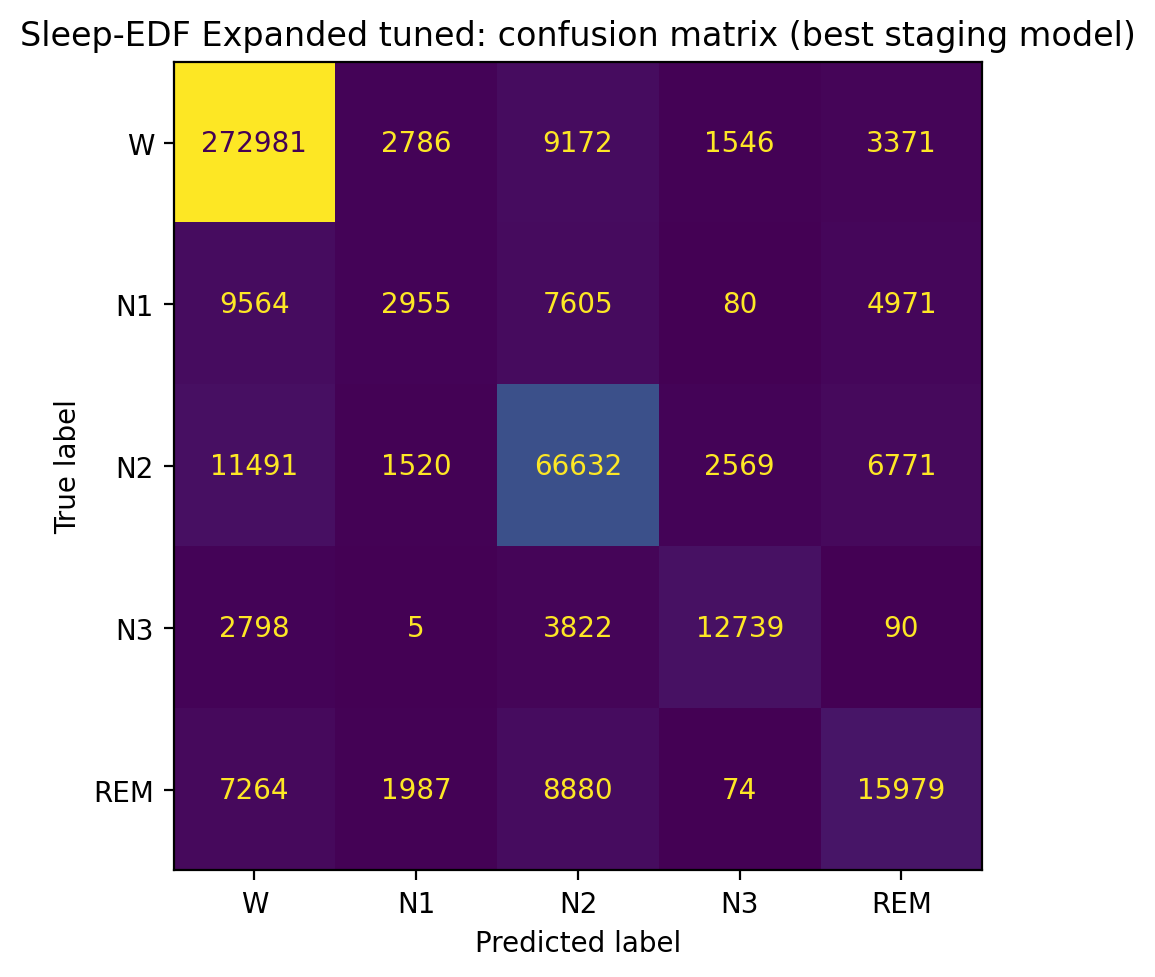
\includegraphics[width=\columnwidth]{sleep_stage_best_confusion.png}
\caption{Matriz de confusi\'on agregada del mejor modelo de staging intra-dataset (XGBoost) en \expname{sleep_edf_expanded_tuned}.}
\label{fig:sleep_stage_confusion}
\end{figure}

La Figura~\ref{fig:sleep_stage_confusion} refuerza un patr\'on ya conocido en la literatura: las mayores confusiones se concentran alrededor de N1 y sus transiciones con W/N2. En cambio, W y N3 resultan m\'as estables, lo cual es coherente con el peso de las \feature{eeg\_*} relacionadas con potencia delta, potencia relativa y cruce por cero.

\subsection{Staging cross-dataset}

\begin{table*}[t]
\centering
\caption{Resultados cross-dataset de staging para las direcciones evaluadas.}
\label{tab:cross_stage}
\resizebox{\textwidth}{!}{%
\begin{tabular}{llccc}
\toprule
Direccion & Modelo & Accuracy & Macro-F1 & Kappa \\
\midrule
Sleep-EDF -> ISRUC & Random Forest & 0.383 & 0.185 & -0.000 \\
Sleep-EDF -> ISRUC & XGBoost & 0.286 & 0.263 & -0.033 \\
Sleep-EDF -> ISRUC & SVM-RBF & 0.277 & 0.273 & -0.026 \\
ISRUC -> Sleep-EDF & Random Forest & 0.477 & 0.308 & 0.046 \\
ISRUC -> Sleep-EDF & XGBoost & 0.209 & 0.192 & -0.051 \\
ISRUC -> Sleep-EDF & SVM-RBF & 0.432 & 0.338 & -0.004 \\
MIT-BIH -> St. Vincent & Random Forest & 0.197 & 0.108 & 0.002 \\
MIT-BIH -> St. Vincent & XGBoost & 0.200 & 0.096 & 0.001 \\
MIT-BIH -> St. Vincent & SVM-RBF & 0.216 & 0.087 & -0.004 \\
St. Vincent -> MIT-BIH & Random Forest & 0.248 & 0.083 & -0.063 \\
St. Vincent -> MIT-BIH & XGBoost & 0.319 & 0.097 & -0.001 \\
St. Vincent -> MIT-BIH & SVM-RBF & 0.063 & 0.024 & 0.000 \\
\bottomrule
\end{tabular}%
}
\end{table*}


La Tabla~\ref{tab:cross_stage} evidencia una ca\'ida severa por cambio de dominio. En la direcci\'on Sleep-EDF \(\rightarrow\) ISRUC, el mejor \emph{accuracy} fue Random Forest con 0.383, pero el mejor \emph{macro-F1} fue SVM-RBF con 0.273. En la direcci\'on ISRUC \(\rightarrow\) Sleep-EDF, Random Forest alcanz\'o la mejor \emph{accuracy} (0.477) y SVM-RBF el mejor \emph{macro-F1} (0.338). En ambos casos, los \emph{kappa} son cercanos a cero o negativos, lo que indica que la generalizaci\'on entre cohortes es d\'ebil incluso cuando el rendimiento bruto parece moderado.

\subsection{MIT-BIH multitarget: apnea + staging}

\begin{table*}[t]
\centering
\caption{MIT-BIH PSG multitarget: media$\pm$desviacion estandar por modelo para apnea y staging.}
\label{tab:mitbih_multitarget}
\resizebox{\textwidth}{!}{%
\begin{tabular}{lccccccc}
\toprule
Modelo & Apnea Acc. & Sens. & Spec. & AUC & Stage Acc. & Stage Macro-F1 & Stage Kappa \\
\midrule
SVM-RBF & 0.576 $\pm$ 0.042 & 0.543 $\pm$ 0.277 & 0.589 $\pm$ 0.166 & 0.600 $\pm$ 0.070 & 0.496 $\pm$ 0.077 & 0.426 $\pm$ 0.054 & 0.336 $\pm$ 0.081 \\
Random Forest & 0.616 $\pm$ 0.039 & 0.458 $\pm$ 0.253 & 0.720 $\pm$ 0.139 & 0.632 $\pm$ 0.071 & 0.585 $\pm$ 0.065 & 0.464 $\pm$ 0.044 & 0.415 $\pm$ 0.078 \\
XGBoost & 0.604 $\pm$ 0.070 & 0.398 $\pm$ 0.250 & 0.761 $\pm$ 0.119 & 0.640 $\pm$ 0.043 & 0.608 $\pm$ 0.040 & 0.446 $\pm$ 0.027 & 0.421 $\pm$ 0.053 \\
\bottomrule
\end{tabular}%
}
\end{table*}

\begin{table}[t]
\centering
\caption{Intervalos de confianza bootstrap para MIT-BIH en apnea (AUC) y staging (accuracy).}
\label{tab:bootstrap_mitbih}
\resizebox{\columnwidth}{!}{%
\begin{tabular}{lcc}
\toprule
Modelo & Apnea AUC-ROC & Stage Accuracy \\
\midrule
SVM-RBF & 0.600 [0.548, 0.655] & 0.496 [0.446, 0.567] \\
Random Forest & 0.632 [0.571, 0.685] & 0.585 [0.537, 0.634] \\
XGBoost & 0.640 [0.609, 0.675] & 0.608 [0.576, 0.640] \\
\bottomrule
\end{tabular}%
}
\end{table}


La Tabla~\ref{tab:mitbih_multitarget} resume el experimento intra-dataset multitarget \expname{mitbih_apnea_stage_classic}. En t\'erminos de media por fold, \textbf{XGBoost} fue el mejor compromiso global: logr\'o el mayor AUC de apnea (\(0.640 \pm 0.043\)) y tambi\'en la mejor \emph{accuracy} de staging (\(0.608 \pm 0.040\)). Sin embargo, \textbf{SVM-RBF} destac\'o en sensibilidad de apnea (\(0.543 \pm 0.277\)), aunque a costa de peor especificidad y menor AUC global. Esto sugiere que el SVM es m\'as proclive a detectar positivos, pero menos estable cuando se eval\'ua discriminaci\'on global.

\begin{figure}[t]
\centering
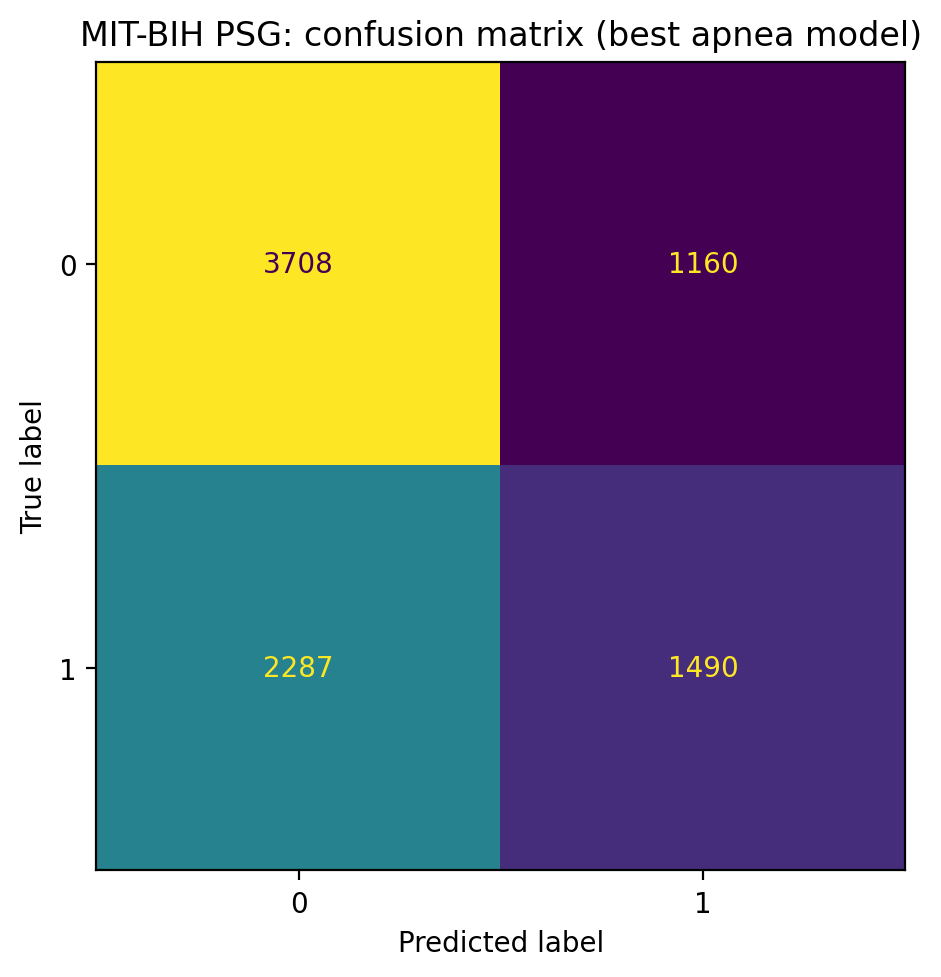
\includegraphics[width=\columnwidth]{mitbih_apnea_best_confusion.png}
\caption{Matriz de confusi\'on agregada del mejor modelo de apnea en MIT-BIH.}
\label{fig:mit_apnea_confusion}
\end{figure}

\begin{figure}[t]
\centering
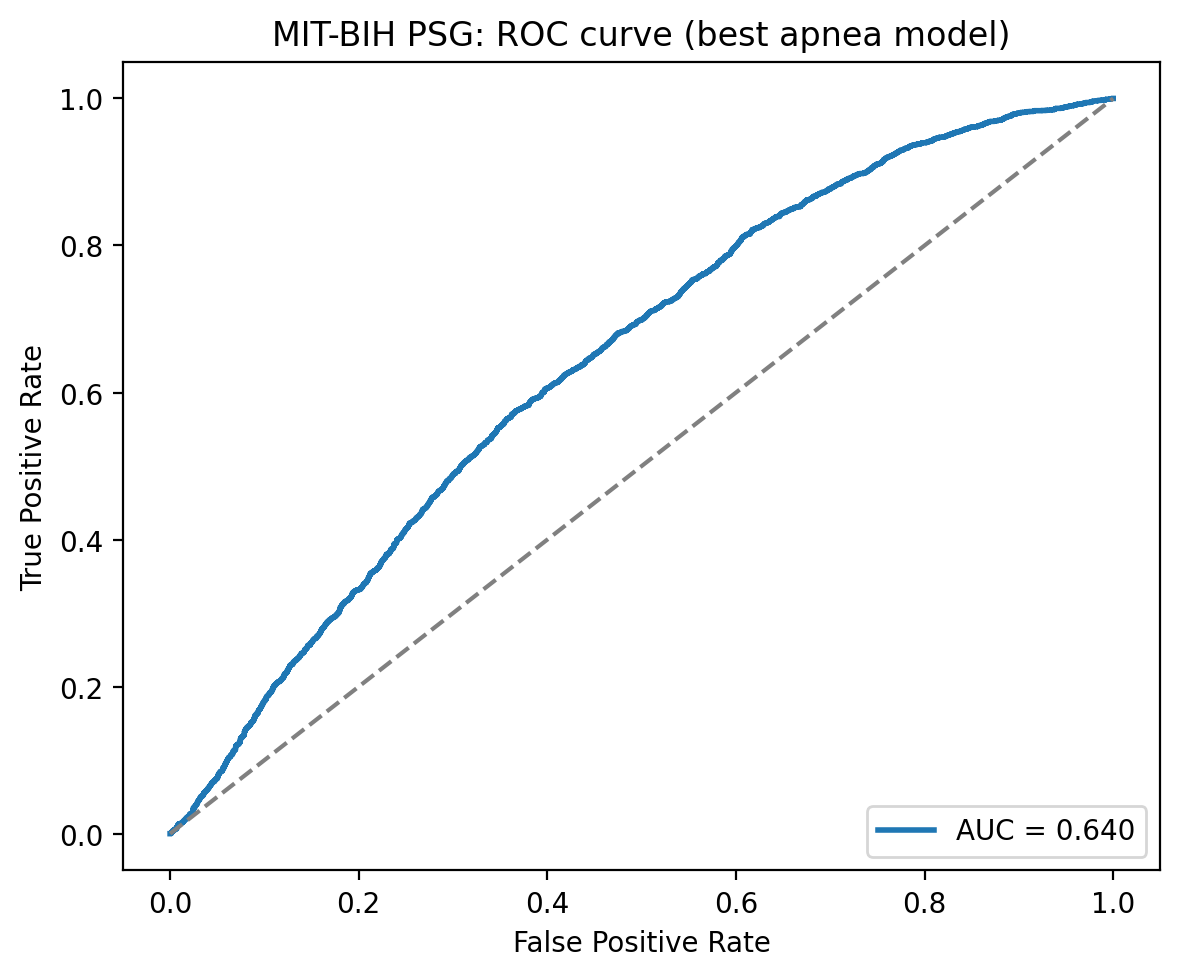
\includegraphics[width=\columnwidth]{mitbih_apnea_best_roc.png}
\caption{Curva ROC agregada del mejor modelo de apnea en MIT-BIH.}
\label{fig:mit_apnea_roc}
\end{figure}

Las Figuras~\ref{fig:mit_apnea_confusion} y \ref{fig:mit_apnea_roc} muestran que el baseline de apnea es razonable como referencia acad\'emica, pero todav\'ia est\'a lejos de una herramienta de despliegue. El rango de AUC intra-dataset ronda 0.60--0.64 y la sensibilidad var\'ia mucho entre folds, se\~nal de que la distribuci\'on de eventos respiratorios sigue siendo un factor cr\'itico.

\subsection{Apnea y staging cross-dataset}

\begin{table*}[t]
\centering
\caption{Resultados cross-dataset de apnea para las direcciones evaluadas.}
\label{tab:cross_apnea}
\resizebox{\textwidth}{!}{%
\begin{tabular}{llcccc}
\toprule
Direccion & Modelo & Accuracy & Sensitivity & Specificity & AUC-ROC \\
\midrule
MIT-BIH -> St. Vincent & Random Forest & 0.741 & 0.106 & 0.900 & 0.528 \\
MIT-BIH -> St. Vincent & XGBoost & 0.799 & 0.000 & 1.000 & 0.452 \\
MIT-BIH -> St. Vincent & SVM-RBF & 0.722 & 0.113 & 0.875 & 0.478 \\
St. Vincent -> MIT-BIH & Random Forest & 0.563 & 0.000 & 1.000 & 0.389 \\
St. Vincent -> MIT-BIH & XGBoost & 0.563 & 0.000 & 1.000 & 0.462 \\
St. Vincent -> MIT-BIH & SVM-RBF & 0.563 & 0.000 & 1.000 & 0.500 \\
\bottomrule
\end{tabular}%
}
\end{table*}


La Tabla~\ref{tab:cross_apnea} deja ver el hallazgo m\'as importante del trabajo: la \textbf{generalizaci\'on cross-dataset para apnea es fr\'agil}. En MIT-BIH \(\rightarrow\) St. Vincent, XGBoost alcanz\'o la mayor \emph{accuracy} (0.799), pero con sensibilidad 0.000 y especificidad 1.000, es decir, una soluci\'on dominada por la clase mayoritaria. En St. Vincent \(\rightarrow\) MIT-BIH el problema es todav\'ia m\'as evidente: los tres modelos obtuvieron sensibilidad 0.000. Este comportamiento confirma que la \emph{accuracy} aislada puede ser enga\~nosa en detecci\'on de apnea.

\subsection{Pruebas estad\'isticas e importancia de variables}

\begin{table*}[t]
\centering
\caption{Pruebas pareadas: McNemar exacto y diferencia bootstrap de AUC.}
\label{tab:stat_tests}
\resizebox{\textwidth}{!}{%
\begin{tabular}{llccc}
\toprule
Escenario & Comparacion & McNemar & p-value & Delta AUC \\
\midrule
Sleep-EDF staging & XGBoost vs Random Forest & 1418.607 & 0.0000 & N/A \\
MIT-BIH staging & XGBoost vs Random Forest & 36.374 & 0.0000 & N/A \\
MIT-BIH apnea & XGBoost vs Random Forest & 8.148 & 0.0043 & -0.011 [-0.016, -0.006] \\
\bottomrule
\end{tabular}%
}
\end{table*}


La Tabla~\ref{tab:stat_tests} a\~nade una capa de interpretaci\'on estad\'istica. En staging intra-dataset y en staging sobre MIT-BIH, la prueba exacta de McNemar entre XGBoost y Random Forest entrega \(p < 0.001\), lo que respalda una diferencia real en sus errores. En apnea sobre MIT-BIH tambi\'en hay diferencia significativa (\(p=0.0043\)), pero la comparaci\'on pareada de AUC produce \(\Delta \mathrm{AUC} = -0.011\;[-0.016,-0.006]\), es decir, el AUC agregado por predicciones fuera de fold favorece levemente a Random Forest. Por tanto, la conclusi\'on sobre ``mejor modelo de apnea'' depende de si se resume por media de folds o por predicciones agregadas.

\begin{figure*}[t]
\centering
\begin{minipage}{0.48\textwidth}
\centering
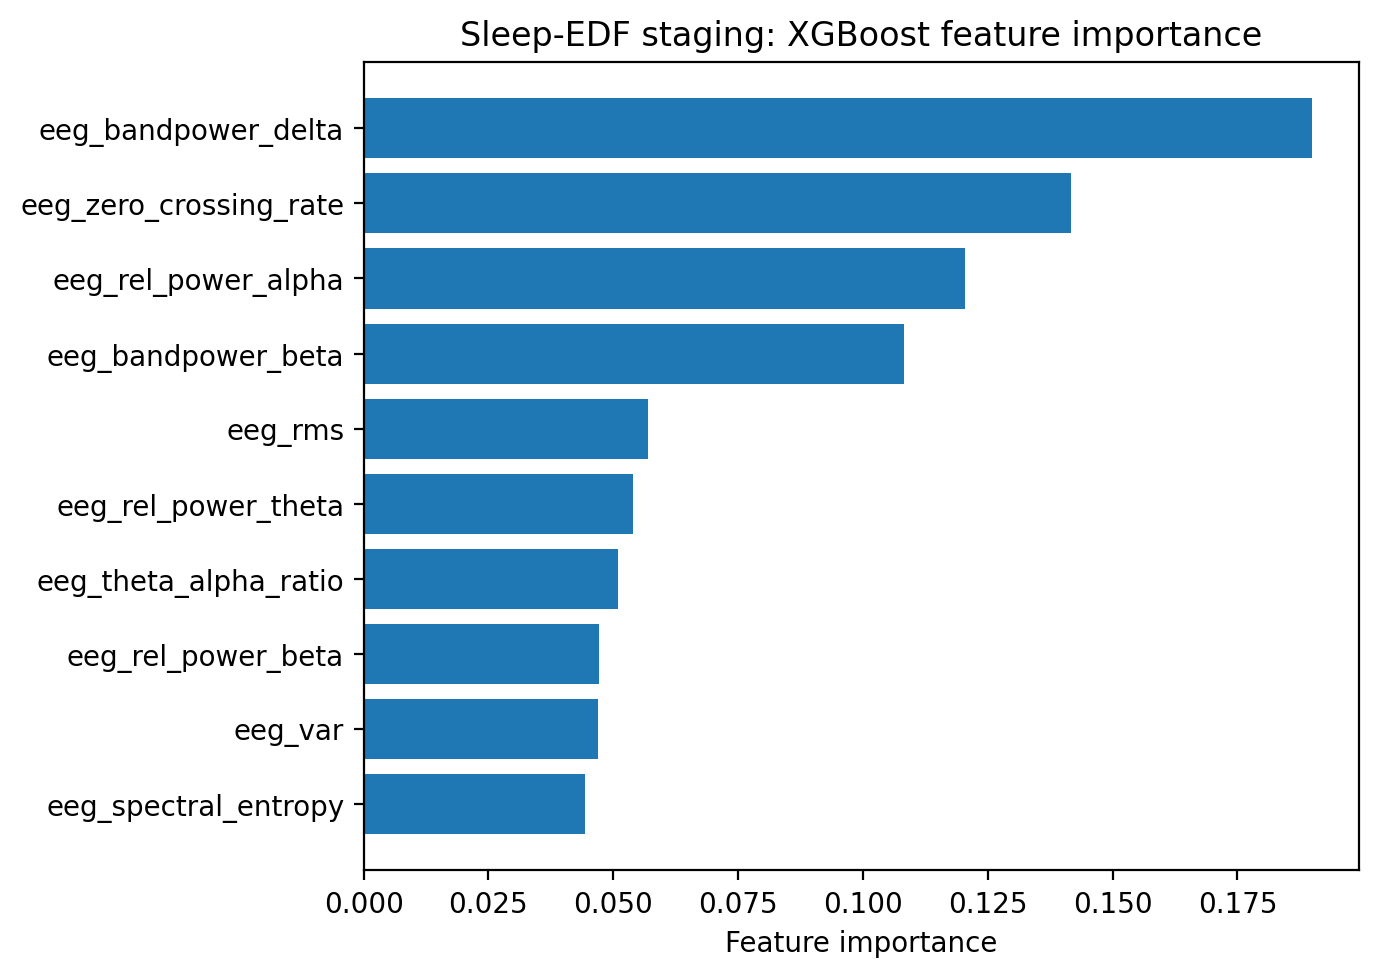
\includegraphics[width=\textwidth]{sleep_stage_xgboost_importance.png}
\end{minipage}
\hfill
\begin{minipage}{0.48\textwidth}
\centering
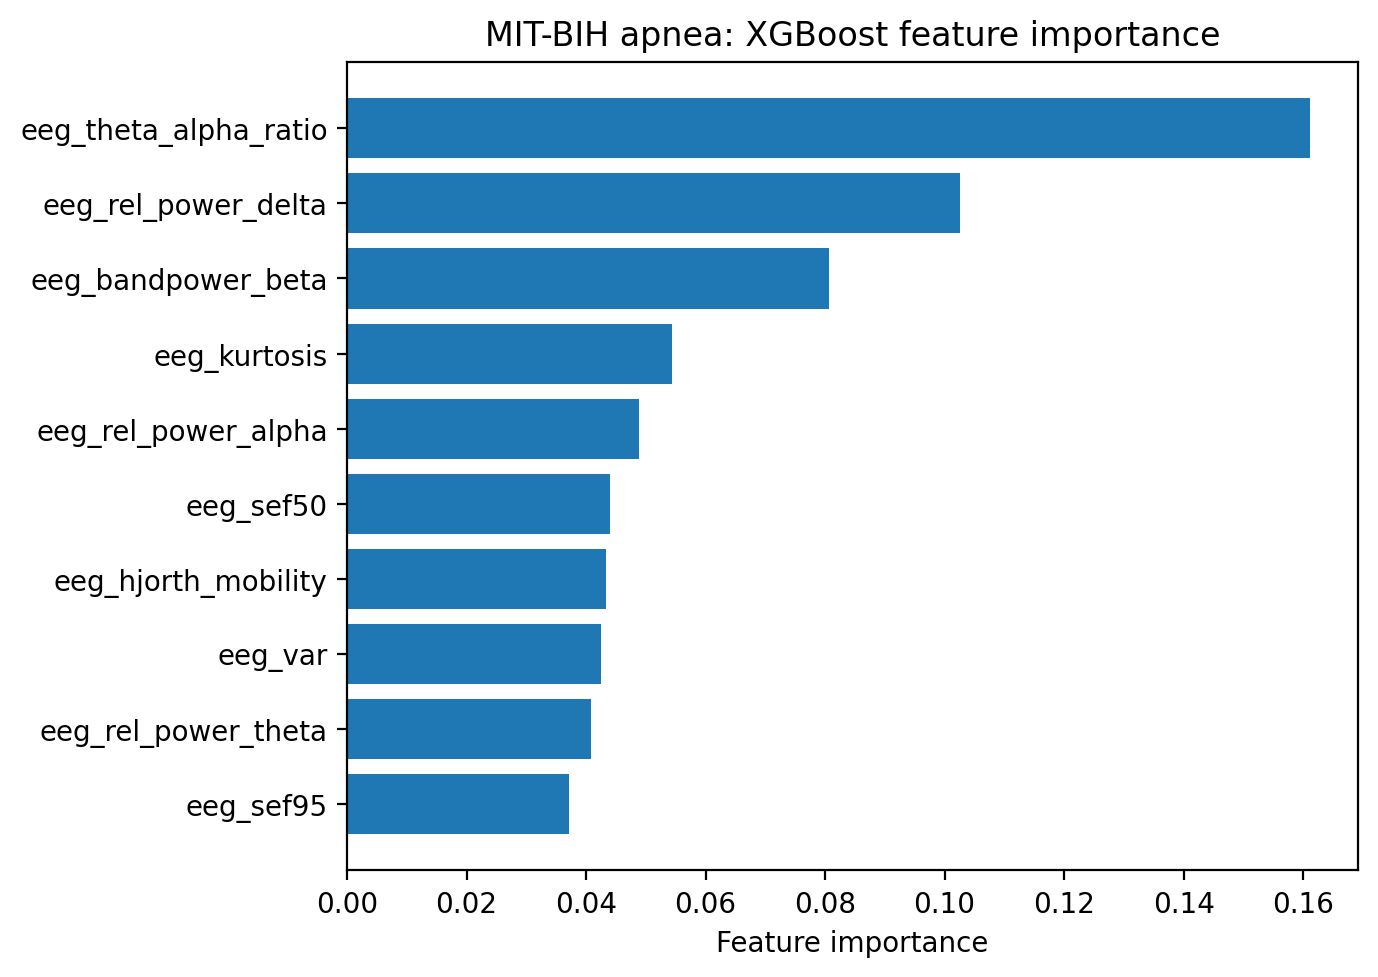
\includegraphics[width=\textwidth]{mitbih_apnea_xgboost_importance.png}
\end{minipage}
\caption{Importancia de variables del mejor modelo de staging en Sleep-EDF (izquierda) y del mejor modelo de apnea en MIT-BIH (derecha).}
\label{fig:feature_importance}
\end{figure*}

La Figura~\ref{fig:feature_importance} muestra que las \feature{eeg\_*} dominantes son coherentes con la fisiolog\'ia del sue\~no: potencia delta, potencia relativa, tasa de cruces por cero, relaci\'on theta/alpha, entrop\'ia espectral y medidas de movilidad/Hjorth. En apnea destacan adem\'as curtosis, SEF50 y SEF95, lo que sugiere sensibilidad a cambios de forma espectral compatibles con micro-despertares y fragmentaci\'on del sue\~no.

\begin{table*}[t]
\centering
\caption{Comparaci\'on resumida entre resultados propios y baselines publicados cercanos.}
\label{tab:published_comparison}
\resizebox{\textwidth}{!}{%
\begin{tabular}{lllll}
\toprule
Referencia & Tarea / dataset & M\'etricas publicadas & Resultado propio m\'as cercano & Nota de comparabilidad \\
\midrule
\cite{mousavi2019sleepeegnet} & Staging, Sleep-EDF & Acc. 0.843; Macro-F1 0.797; $\kappa=0.79$ & XGBoost: Acc. 0.811; RF: Macro-F1 0.608; XGBoost: $\kappa=0.644$ & Ellos usan modelo profundo con contexto secuencial \\
\cite{gao2023psdrf} & Staging, Sleep-EDF & Acc. 0.919; Macro-F1 0.732; $\kappa=0.845$ & RF: Acc. 0.796; Macro-F1 0.608; $\kappa=0.631$ & Muy comparable por dataset/canal, pero protocolo no necesariamente igual \\
\cite{nakamura2017complexity} & Staging, Sleep-EDF Expanded & Acc. 0.938; sensibilidad S1 0.491; $\kappa=0.90$ & XGBoost: Acc. 0.811; N1 F1 0.171; RF: N1 F1 0.256 & Nuestro protocolo es m\'as conservador y no usa contexto expl\'icito \\
\cite{barnes2022apneaeegcnn} & Apnea, EEG monocanal & Acc. 0.699; MCC 0.38 & XGBoost MIT-BIH: Acc. 0.604; AUC 0.640 & Cohortes y m\'etricas no son id\'enticas, pero la tarea y la restricci\'on de canal s\'i \\
\bottomrule
\end{tabular}%
}
\end{table*}


Finalmente, la Tabla~\ref{tab:published_comparison} compara nuestros resultados con baselines publicados cercanos. Los n\'umeros propios son m\'as conservadores que varios reportes de la literatura, lo cual es esperable dado que aqu\'i se mantuvo una partici\'on \emph{subject-wise} estricta y una misma disciplina metodol\'ogica para todos los modelos.

\section{An\'alisis y discusi\'on}

Los resultados permiten una lectura clara. Dentro de dataset, la l\'inea cl\'asica sobre EEG monocanal s\'i alcanza baselines defendibles. Fuera de dataset, el rendimiento cae de forma abrupta, en especial para apnea. Por eso la contribuci\'on principal del trabajo no es solo reportar ``qu\'e modelo gan\'o'', sino mostrar c\'omo cambian las conclusiones al pasar de \emph{accuracy} a \emph{macro-F1}, de media por fold a contraste pareado, y de validaci\'on interna a generalizaci\'on externa.

\subsection{Respuestas a las preguntas de an\'alisis}

\begin{enumerate}[leftmargin=*]
\item \textbf{¿Qu\'e combinaci\'on de preprocesamiento + \emph{features} produjo el mejor resultado y por qu\'e cree que funcion\'o mejor?} La mejor combinaci\'on para staging fue la de ventanas de 30 s, estandarizaci\'on ajustada dentro de cada fold y \feature{eeg\_*} espectrales compactas, especialmente potencia delta, potencias relativas, \emph{zero-crossing rate} y entrop\'ia espectral. En apnea funcion\'o mejor la versi\'on extendida con Hjorth, SEF50/95, entrop\'ias y curtosis. Esa mezcla funciona porque separa tanto macroestados de sue\~no como cambios finos de microestructura que suelen acompa\~nar eventos respiratorios.

\item \textbf{¿Qu\'e tan sensible fue cada modelo al desbalance de clases, especialmente en N1 o en apnea/no-apnea?} Fue muy sensible. En staging, N1 fue la clase m\'as castigada: el mejor F1 de N1 en Sleep-EDF fue apenas 0.256 con Random Forest, mientras que W super\'o 0.91 (Tabla~\ref{tab:stage_f1_class}). En apnea, el desbalance se vuelve cr\'itico en \emph{cross-dataset}: por ejemplo, MIT-BIH \(\rightarrow\) St. Vincent da una \emph{accuracy} de 0.799 con XGBoost, pero sensibilidad 0.000, un patr\'on cl\'asico de sesgo hacia la clase mayoritaria.

\item \textbf{¿Qu\'e diferencias observa entre \emph{accuracy}, \emph{macro-F1} y \emph{kappa}? ¿Alg\'un modelo parece ``bueno'' solo porque favorece clases mayoritarias?} S\'i. XGBoost fue el mejor en \emph{accuracy} y \emph{kappa} intra-dataset sobre Sleep-EDF, pero Random Forest fue mejor en \emph{macro-F1}. Eso indica que el mejor promedio global no coincide necesariamente con el mejor equilibrio entre clases. En apnea \emph{cross-dataset}, la \emph{accuracy} alta con sensibilidad cero demuestra de forma extrema que un modelo puede parecer ``bueno'' solo por predecir la clase negativa dominante.

\item \textbf{¿Qu\'e patrones aparecen en las matrices de confusi\'on? ¿Qu\'e clases se confunden con mayor frecuencia y por qu\'e?} La matriz de confusi\'on de Sleep-EDF (Figura~\ref{fig:sleep_stage_confusion}) muestra que N1 se mezcla con N2 y con vigilia. Esto tiene sentido porque N1 es una etapa transicional y, con EEG monocanal, su firma es menos estable que la de N3 o W. En apnea, la matriz de MIT-BIH confirma una cantidad importante de falsos negativos, se\~nal de que el modelo identifica mejor ausencia de evento que presencia de evento.

\item \textbf{¿El mejor modelo dentro de un dataset tambi\'en fue el mejor en \emph{cross-dataset}? Si no, ¿qu\'e indica eso sobre generalizaci\'on?} No. XGBoost domina dentro de Sleep-EDF y MIT-BIH cuando se mira rendimiento agregado interno, pero en staging \emph{cross-dataset} SVM-RBF obtuvo el mejor \emph{macro-F1} en ambas direcciones Sleep-EDF/ISRUC. Esto indica que el mejor ajuste intra-dataset no garantiza robustez fuera de dominio; probablemente algunos modelos est\'an explotando regularidades espec\'ificas del corpus fuente.

\item \textbf{¿Qu\'e tanto cambi\'o el rendimiento al pasar de \emph{epoch-wise} impl\'icito a \emph{subject-wise} estricto? ¿Existe evidencia de fuga de informaci\'on en alg\'un dise\~no preliminar?} Nuestros resultados son m\'as bajos que varios papers que reportan 0.84--0.94 de \emph{accuracy} en Sleep-EDF \cite{mousavi2019sleepeegnet,gao2023psdrf,nakamura2017complexity}. Esa brecha es consistente con el endurecimiento del protocolo: particiones \emph{subject-wise} estrictas, tuning solo en train y una disciplina uniforme entre datasets. No se presenta evidencia de fuga en la versi\'on final, pero la diferencia con la literatura sugiere que dise\~nos menos estrictos pueden inflar el rendimiento.

\item \textbf{¿Los intervalos de confianza de dos modelos se superponen? ¿Eso cambia su conclusi\'on sobre cu\'al es realmente mejor?} S\'i. En Sleep-EDF, los IC bootstrap de \emph{macro-F1} de Random Forest y XGBoost se superponen de forma importante (Tabla~\ref{tab:bootstrap_sleep_stage}), aunque el \emph{accuracy} de XGBoost queda ligeramente por encima. En MIT-BIH, los IC de AUC de Random Forest y XGBoost tambi\'en se superponen ampliamente. Esto obliga a una conclusi\'on matizada: XGBoost es el mejor compromiso global, pero no por un margen tan amplio como para descartar por completo a Random Forest.

\item \textbf{¿McNemar o la comparaci\'on de AUC apoyan una diferencia significativa o la mejora observada es solo marginal?} Para staging, McNemar respalda diferencias reales entre XGBoost y Random Forest tanto en Sleep-EDF como en MIT-BIH (Tabla~\ref{tab:stat_tests}). Para apnea en MIT-BIH tambi\'en hay diferencia significativa por McNemar (\(p=0.0043\)). Sin embargo, la diferencia bootstrap pareada de AUC favorece levemente a Random Forest sobre las predicciones agregadas. Por tanto, la mejora de XGBoost en apnea no es absoluta; depende de c\'omo se agregue la evidencia.

\item \textbf{¿Qu\'e \emph{features} resultaron m\'as importantes seg\'un RF/boosting? ¿Tienen sentido fisiol\'ogico o solo parecen estad\'isticamente \'utiles?} En staging dominaron \feature{eeg\_bandpower\_delta}, \feature{eeg\_zero\_crossing\_rate}, \feature{eeg\_rel\_power\_alpha}, \feature{eeg\_bandpower\_beta} y \feature{eeg\_spectral\_entropy}. En apnea destacaron \feature{eeg\_theta\_alpha\_ratio}, \feature{eeg\_rel\_power\_delta}, \feature{eeg\_bandpower\_beta}, \feature{eeg\_kurtosis}, \feature{eeg\_sef50} y \feature{eeg\_hjorth\_mobility}. Esas variables s\'i tienen sentido fisiol\'ogico: recogen lentificaci\'on cortical, fragmentaci\'on y cambios de estructura espectral asociados a etapas y a micro-arousals.

\item \textbf{¿C\'omo afecta el ruido, la presencia de artefactos o el cambio de base de datos al desempe\~no del modelo?} El efecto es fuerte. La ca\'ida entre intra-dataset y \emph{cross-dataset} es demasiado grande para atribuirla solo al azar. Adem\'as, no hubo un m\'odulo expl\'icito de rechazo de artefactos cl\'inicos; el pipeline conf\'ia en canalizaci\'on, remuestreo y \emph{features} robustas. Por eso el ruido residual, la diferencia de cohortes y la no equivalencia exacta del canal EEG aparecen reflejados directamente en la degradaci\'on del rendimiento.

\item \textbf{¿SVM super\'o o no a RF/boosting? Explique la raz\'on en t\'erminos de separaci\'on no lineal, tama\~no del conjunto y estabilidad.} En t\'erminos globales, no. SVM no fue el mejor baseline intra-dataset y qued\'o claramente por debajo en MIT-BIH multitarget. No obstante, en staging \emph{cross-dataset} obtuvo el mejor \emph{macro-F1}, lo que sugiere que su frontera radial sobre un conjunto compacto de \feature{eeg\_*} puede ser menos sobreajustada que la de los ensambles en ciertos dominios. Aun as\'i, RF y XGBoost fueron m\'as estables y m\'as consistentes a lo largo de la bater\'ia completa.

\item \textbf{¿Qu\'e baseline publicado es el m\'as comparable con su experimento y en qu\'e aspectos la comparaci\'on todav\'ia no es totalmente justa?} Para staging, el baseline m\'as comparable es Gao y Wu \cite{gao2023psdrf}, porque comparte Sleep-EDF, EEG monocanal y Random Forest con \emph{features} espectrales. Para apnea, el referente m\'as cercano es Barnes \emph{et al.} \cite{barnes2022apneaeegcnn}, por su restricci\'on a EEG monocanal y su foco expl\'icito en apnea. La comparaci\'on no es totalmente justa porque cambian cohortes, protocolo de partici\'on, definici\'on de labels, posibles estrategias de balance y, en algunos casos, el propio canal EEG.

\item \textbf{Si tuviera que desplegar el sistema en un escenario real con un EEG simple, ¿qu\'e modelo elegir\'ia y por qu\'e?} Elegir\'ia \textbf{XGBoost} como punto de partida, porque fue el mejor compromiso global en el paquete final: mejor \emph{accuracy}/\emph{kappa} de staging en Sleep-EDF y mejor balance medio apnea+staging en MIT-BIH. Sin embargo, no lo desplegar\'ia sin recalibraci\'on externa, ajuste de umbral y validaci\'on adicional en una cohorte destino, porque los experimentos \emph{cross-dataset} muestran que ninguno de los tres modelos es todav\'ia robusto fuera del dominio fuente.
\end{enumerate}

\section{Propuesta de mejora}

La limitaci\'on dominante de la bater\'ia experimental es el \textbf{cambio de dominio}. Por ello, la mejora propuesta no apunta a exprimir unas d\'ecimas extra dentro del mismo dataset, sino a aumentar la robustez \emph{cross-dataset}. La propuesta concreta es un \textbf{Conformer multitarea con adaptaci\'on adversarial de dominio} para EEG monocanal, entrenado con las mismas ventanas de 30 s y con dos cabezas: una para \texttt{sleep\_stage} y otra para \texttt{apnea\_binary}. La tercera cabeza ser\'ia un discriminador de dominio que intenta identificar si una ventana proviene del corpus fuente o del corpus destino.

\subsection{Justificaci\'on te\'orica}

La idea es aprender una representaci\'on del EEG que conserve informaci\'on discriminativa para staging y apnea, pero que sea lo menos sensible posible a la identidad del dataset. Si el encoder se entrena con una p\'erdida de clasificaci\'on multitarea y, simult\'aneamente, con una p\'erdida adversarial que penaliza la separabilidad fuente/destino, entonces parte del sesgo por cohorte podr\'ia reducirse sin abandonar la restricci\'on de EEG monocanal. Esta propuesta ataca directamente el principal hallazgo del trabajo: el deterioro radical de las m\'etricas cuando el modelo sale del dataset fuente.

\subsection{Pseudoc\'odigo}

\begin{quote}
\ttfamily
Entrada: ventanas EEG monocanal de 30 s, etiquetas de staging/apnea en el dominio fuente,\\
ventanas sin etiquetar o parcialmente etiquetadas en el dominio destino.\\[4pt]
1. Extraer secuencias de \'epocas desde el mismo contrato temporal usado en la l\'inea cl\'asica.\\
2. Pasar cada secuencia por un encoder Conformer compartido.\\
3. Alimentar la representaci\'on latente a: (a) cabeza de staging, (b) cabeza de apnea.\\
4. Alimentar la misma representaci\'on a un discriminador de dominio con gradiente invertido.\\
5. Optimizar una p\'erdida total = p\'erdida\_stage + lambda\_a * p\'erdida\_apnea - lambda\_d * p\'erdida\_dominio.\\
6. Ajustar s\'olo con train del dominio fuente y datos no etiquetados del destino.\\
7. Evaluar con el mismo protocolo subject-wise y cross-dataset del baseline cl\'asico.
\end{quote}

\subsection{Evaluaci\'on justa frente al baseline}

Para que la comparaci\'on sea justa, el m\'etodo propuesto deber\'ia:
\begin{itemize}[leftmargin=*]
\item usar exactamente los mismos sujetos fuente/destino que la bater\'ia final de este informe;
\item mantener EEG monocanal y ventanas de 30 s;
\item no ajustar hiperpar\'ametros con etiquetas del conjunto destino;
\item reportar las mismas m\'etricas de apnea y staging;
\item compararse contra el mejor baseline cl\'asico de este trabajo, no contra un baseline m\'as d\'ebil.
\end{itemize}

La propuesta es factible, est\'a alineada con el patr\'on de error observado y responde al problema metodol\'ogico central del laboratorio: lograr robustez entre cohortes heterog\'eneas sin abandonar la simplicidad instrumental del EEG monocanal.

\section{Conclusiones y trabajo futuro}

Este informe cerr\'o la bater\'ia m\'inima del laboratorio sin bono con seis experimentos reproducibles y una l\'inea principal cl\'asica sobre EEG monocanal. Los resultados permiten tres conclusiones principales. Primero, dentro de dataset, la combinaci\'on de ventanas de 30 s, \feature{eeg\_*} espectrales/de complejidad y ensambles basados en \'arboles ofrece baselines s\'olidos. En Sleep-EDF, XGBoost fue el mejor por \emph{accuracy} y \emph{kappa}, mientras que Random Forest fue el mejor por \emph{macro-F1}. En MIT-BIH multitarget, XGBoost fue el mejor compromiso medio entre apnea y staging.

Segundo, el principal problema no es la optimizaci\'on interna sino la \textbf{generalizaci\'on}. Todos los experimentos \emph{cross-dataset} mostraron degradaciones fuertes. En apnea, incluso aparecieron soluciones con sensibilidad nula y especificidad perfecta, una combinaci\'on inaceptable para despliegue real aunque la \emph{accuracy} parezca alta. Por ello, el hallazgo m\'as importante del trabajo es que los baselines cl\'asicos son \'utiles como referencia reproducible, pero no bastan por s\'i solos para sostener transferencia entre cohortes.

Tercero, el an\'alisis m\'etrico confirma que no basta con mirar \emph{accuracy}. La baja F1 de N1, la sensibilidad inestable de apnea, la superposici\'on parcial de intervalos de confianza y la discrepancia entre media de folds y AUC agregada muestran que las conclusiones deben ser matizadas y apoyarse en varias evidencias a la vez.

Como trabajo futuro se proponen tres l\'ineas directas: incorporar un m\'odulo expl\'icito de manejo de artefactos, extender el an\'alisis a severidad cl\'inica por paciente cuando el \emph{ground truth} sea consistente, e implementar una estrategia de adaptaci\'on de dominio para EEG monocanal. Esa tercera l\'inea es la m\'as prometedora, porque ataca precisamente el cuello de botella que la bater\'ia experimental final dej\'o al descubierto.


\appendices
\section{Comandos de ejecuci\'on}

La bater\'ia final del informe se reproduce con los siguientes comandos, asumiendo el entorno virtual activado en la ra\'iz del repositorio:

\begin{itemize}[leftmargin=*]
\item \texttt{python scripts/run\_phase\_e\_cv.py}\\
\texttt{\ \ --config config/experiments/sleep\_edf\_expanded\_tuned.yaml}
\item \texttt{python scripts/run\_phase\_e\_cv.py}\\
\texttt{\ \ --config config/experiments/cross\_sleep\_edf\_to\_isruc\_n123.yaml}
\item \texttt{python scripts/run\_phase\_e\_cv.py}\\
\texttt{\ \ --config config/experiments/cross\_isruc\_to\_sleep\_edf\_n123.yaml}
\item \texttt{python scripts/run\_phase\_e\_classic\_multitarget.py}\\
\texttt{\ \ --config config/experiments/mitbih\_apnea\_stage\_classic.yaml}
\item \texttt{python scripts/run\_phase\_e\_classic\_multitarget.py}\\
\texttt{\ \ --config config/experiments/cross\_dataset\_mitbih\_to\_st\_vincent\_classic.yaml}
\item \texttt{python scripts/run\_phase\_e\_classic\_multitarget.py}\\
\texttt{\ \ --config config/experiments/cross\_dataset\_st\_vincent\_to\_mitbih\_classic.yaml}
\end{itemize}

Para construir el informe:

\begin{itemize}[leftmargin=*]
\item \texttt{python scripts/build\_latex\_report\_assets.py}
\item \texttt{cd report/latex}
\item \texttt{pdflatex --disable-installer -interaction=nonstopmode -halt-on-error main.tex}
\item \texttt{bibtex main}
\item \texttt{pdflatex --disable-installer -interaction=nonstopmode -halt-on-error main.tex}
\item \texttt{pdflatex --disable-installer -interaction=nonstopmode -halt-on-error main.tex}
\end{itemize}

Tambi\'en se dej\'o un script de conveniencia en \texttt{report/latex/build\_report.ps1}.

\section{Uso de herramientas de IA}

Durante el proyecto se utilizaron herramientas de IA para tres tareas: (1) exploraci\'on y depuraci\'on de c\'odigo, (2) apoyo en la estructuraci\'on del informe y (3) apoyo en la s\'intesis inicial de literatura. Todo resultado incluido en el informe fue verificado manualmente contra archivos reales del repositorio o contra PDFs/fuentes bibliogr\'aficas consultadas.

\begin{table}[h]
\centering
\caption{Uso declarado de herramientas de IA.}
\label{tab:ai_use}
\resizebox{\columnwidth}{!}{%
\begin{tabular}{lll}
\toprule
Herramienta & Uso principal & Verificaci\'on manual \\
\midrule
Codex / GPT-5.4 & C\'odigo, refactor, LaTeX & S\'i \\
ChatGPT/Codex & Redacci\'on y s\'intesis & S\'i \\
PDF local / revisi\'on manual & Literatura base & S\'i \\
\bottomrule
\end{tabular}%
}
\end{table}

No se incluyeron referencias inventadas, m\'etricas no ejecutadas ni figuras no trazables a artefactos del proyecto.


\bibliographystyle{IEEEtran}
\bibliography{references}

\end{document}
